\begin{frame}
    \frametitle{The empirical Bayes model, part 1}
    \begin{center}
        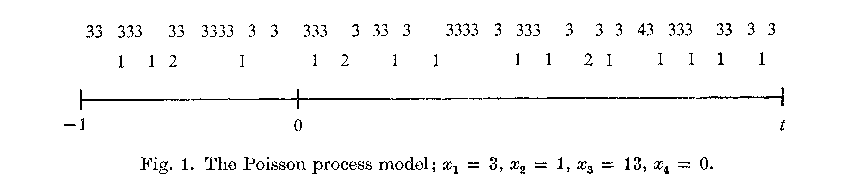
\includegraphics[width=4in]{../compendium/Figures/ET-Figure1.pdf}        
    \end{center}
	\begin{enumerate}
		\item Species $s$ is ``trapped'' according to a Poisson$(\lambda_s)$ process
		\item Species $s$ appears $x_s=x_s(t)$ times in $[-1,t]$, so that
		\item $x_s(t) \sim \mathsf{Poisson}(\lambda_s(1+t))$, and
		\item Observed data = $\{x_s\}$, where $x_s\equiv x_s(0)$
	\end{enumerate}

\end{frame}

\begin{frame}
    \frametitle{The empirical Bayes model, part 2}
	Let $G(\lambda)$ be the cdf of $\{\lambda_s \vert s=1,\dots,S\}$. Then:
	\begin{equation}
		\eta_x = \E(n_x) = S\int_0^\infty (e^{-\lambda}\lambda^x/x!)\,dG(\lambda).
		\label{eq:eta}
	\end{equation}
	
	
	The expected number of species (words) seen for the first time in $(0,t]$ is
	\begin{equation}
		\Delta(t) = S\int_0^\infty e^{-\lambda}(1-e^{-\lambda t})\,dG(\lambda)
		\label{eq:delta}
	\end{equation}
	
	Expanding $1-e^{-\lambda t}$ in (\ref{eq:delta}) and comparing to (\ref{eq:eta}), we have formally
	\begin{equation}
		\Delta(t) = \eta_1 t-\eta_2 t^2 + \eta_3 t^3 - \ldots\ .
	\end{equation}
\end{frame}

\begin{frame}
	\frametitle{An observation}
	\begin{center}
		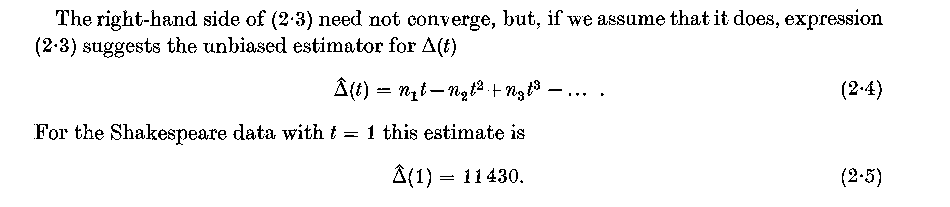
\includegraphics[width=4.5in]{../compendium/Figures/ET-eqns-(2_4)-and-(2_5).pdf}
	\end{center}
\end{frame}

\begin{frame}
    \frametitle{Fisher's negative binomial model}
	Take $G(\lambda)$ to have a gamma density
	$$g_{\alpha\beta}(\lambda) \propto \lambda^{\alpha-1}e^{-\lambda/\beta}.$$
	
	Then from (\ref{eq:eta}) we have
	\begin{equation}
		\eta_x = \eta_1{\Gamma(x+\alpha)\over x!\,\Gamma(1+\alpha)}\gamma^{x-1}, \quad\mbox{where\ } \gamma = {\beta \over 1+\beta}.
		\label{eq:fisher}
	\end{equation}
	
	After some manipulation, we get a parametric expression for $\Delta(t):$
	\begin{equation}
		\Delta_{\alpha\gamma}(t) = -\eta_1{(1+\gamma t)^{-\alpha}-1 \over \gamma\,\alpha}.
		\label{eq:deltaAG}
	\end{equation}
\end{frame}
